\section{VisPerf}

Since Perf can output a lot of data, we propose VisPerf to easily visualize and compare the data captured. The VisPerf pipeline can be seen as three stages: capture, pre-processing and visualization.

In the capture stage, the person recognition stream application is executed using the mapping policies from operating system and FastFlow, and profiled with Perf. We configured Perf to sample 997 captures each second the application is running. The raw data from Perf is converted to a CSV file for posterior analysis.

In the second stage, the CSV files are processed and merged. In summary, the processing phase groups captures made inside the same second, extract the three top functions in the stack executing on the CPU, and also setting the label to the threads. This stage generates a JSON file that is upload to VisPerf dashboard for human analysis. The JSON file contains the structured data of each experiment and also the details of the hardware where experiments where executed, enabling fast data reading on the VisPerf dashboard. Moreover, generating a single JSON file with all experiment makes it simple to share data for analysis between researchers.

After these two stages finished, VisPerf can be to analyze data captured. In Section~\ref{section:visualization-interaction}, we discuss the visualizations and interactions we propose for VisPerf.


\subsection{Visualizations and Interactions} \label{section:visualization-interaction}

The first step inside VisPerf is to upload the JSON file generated in the second stage. VisPerf reads this file and generate the plots. We used D3\footnote{\url{https://d3js.org}} library to create the visualizations, since it is very customizable and with many features to allow users to interact with the plots. Since the JSON file file may contains many experiments, we allow the user to select which experiments they want to compare. The user can select up to two experiments.

VisPerf visualization is divided into three sections. The first section, showed in Figure~\ref{figure:vispef-section-1}, is named ``Comparing experiments''. This section compares specific events captured while executing the two experiments selected. As shown in Figure~\ref{figure:visperf-section-1}, the user can select the event to be compared and the plot. For this sections, there are two plots available: the parallel coordinates and another plot with a grid representing the CPUs available in the processor where experiments were executed.

\begin{figure}
    \centering
    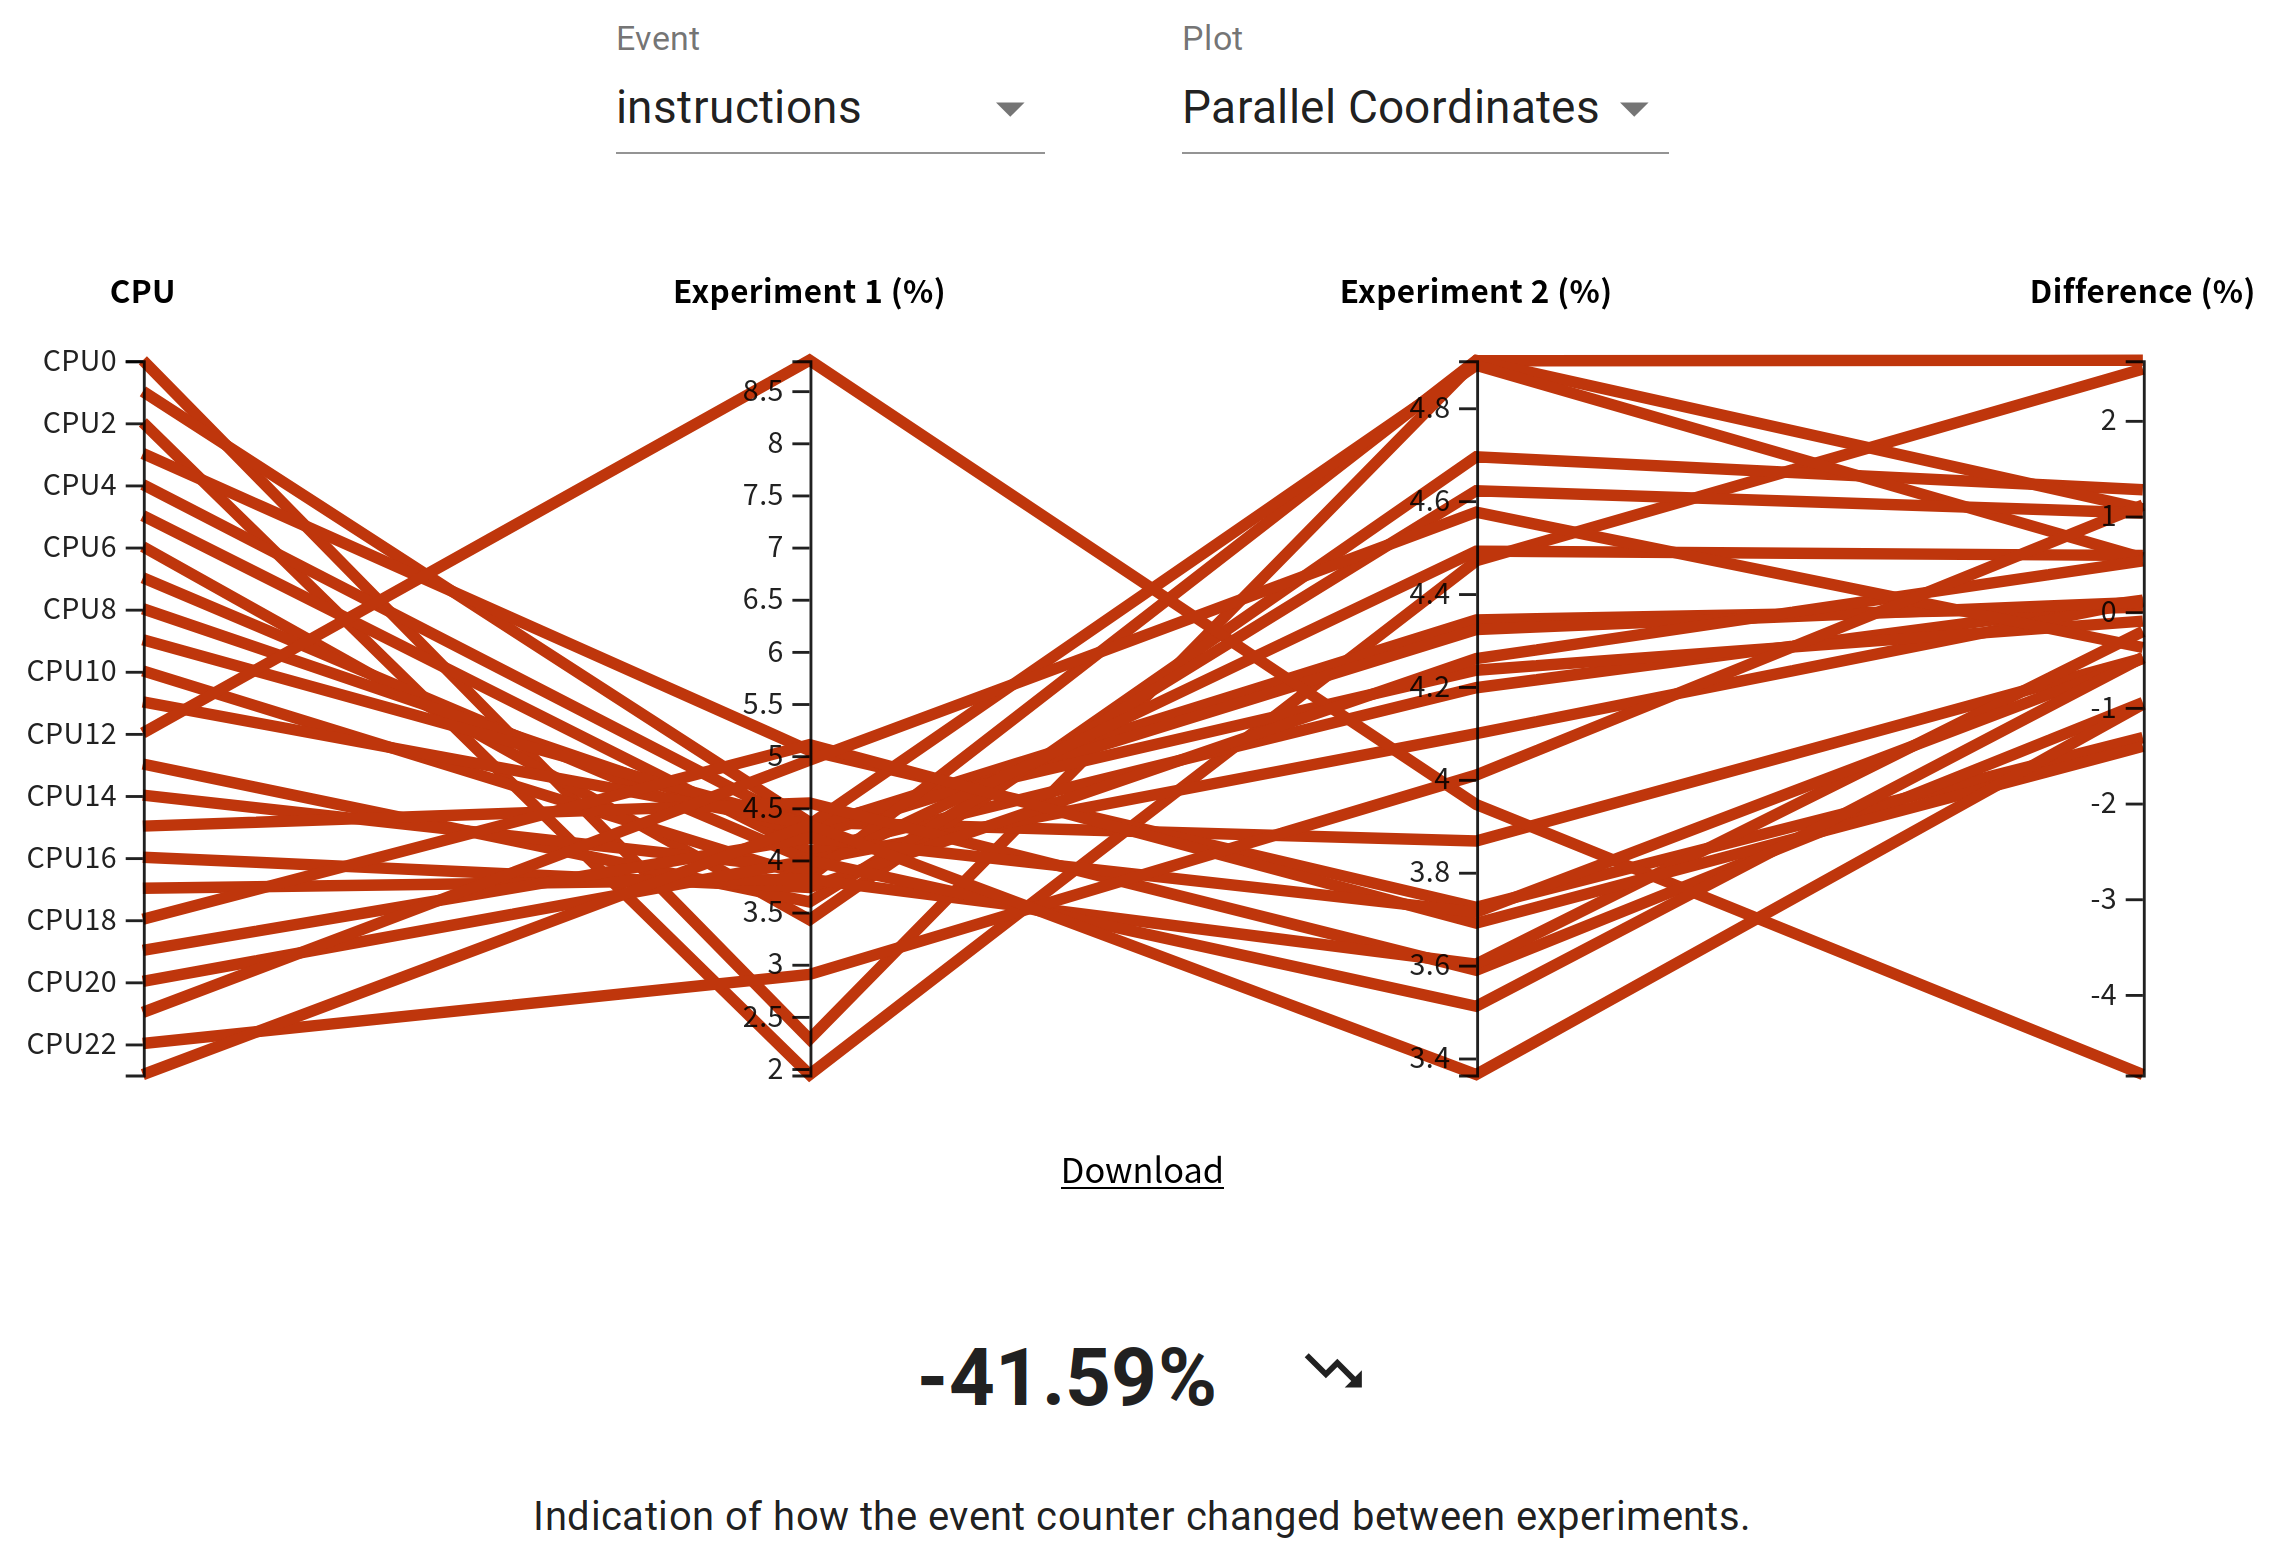
\includegraphics[width=1.0\columnwidth]{../pictures/visperf-section-1.png}
    \caption{VisPerf section ``Comparing experiments''.}
    \label{figure:visperf-section-1}
\end{figure}

The first section in VisPerf also shows a summary of how the event selected change between the experiments. As shows in Figure~\ref{figure:visperf-section-1}, the second experiment needed 41.59\% less instructions to finish the execution. Another important metric that this plot can shows is that the second experiment had a better balance between the CPUs. CPU 12, for example, executed $\approx$ 9\% of the instructions, while in experiment two the most CPUs executed $\approx$ 5\% of the instructions. The last columns in the parallel coordinates plots shows the absolute difference between the CPUs.

The parallel coordinate plots seems to be a little messy because of the high number of lines. However, when hovering a specific line, this line is highlighted and the opacity of other lines diminished. Another feature that is present in all plots is the download button. Here the plot is save in SVG format, that can be converted to any other format by the user.

\begin{figure}
    \centering
    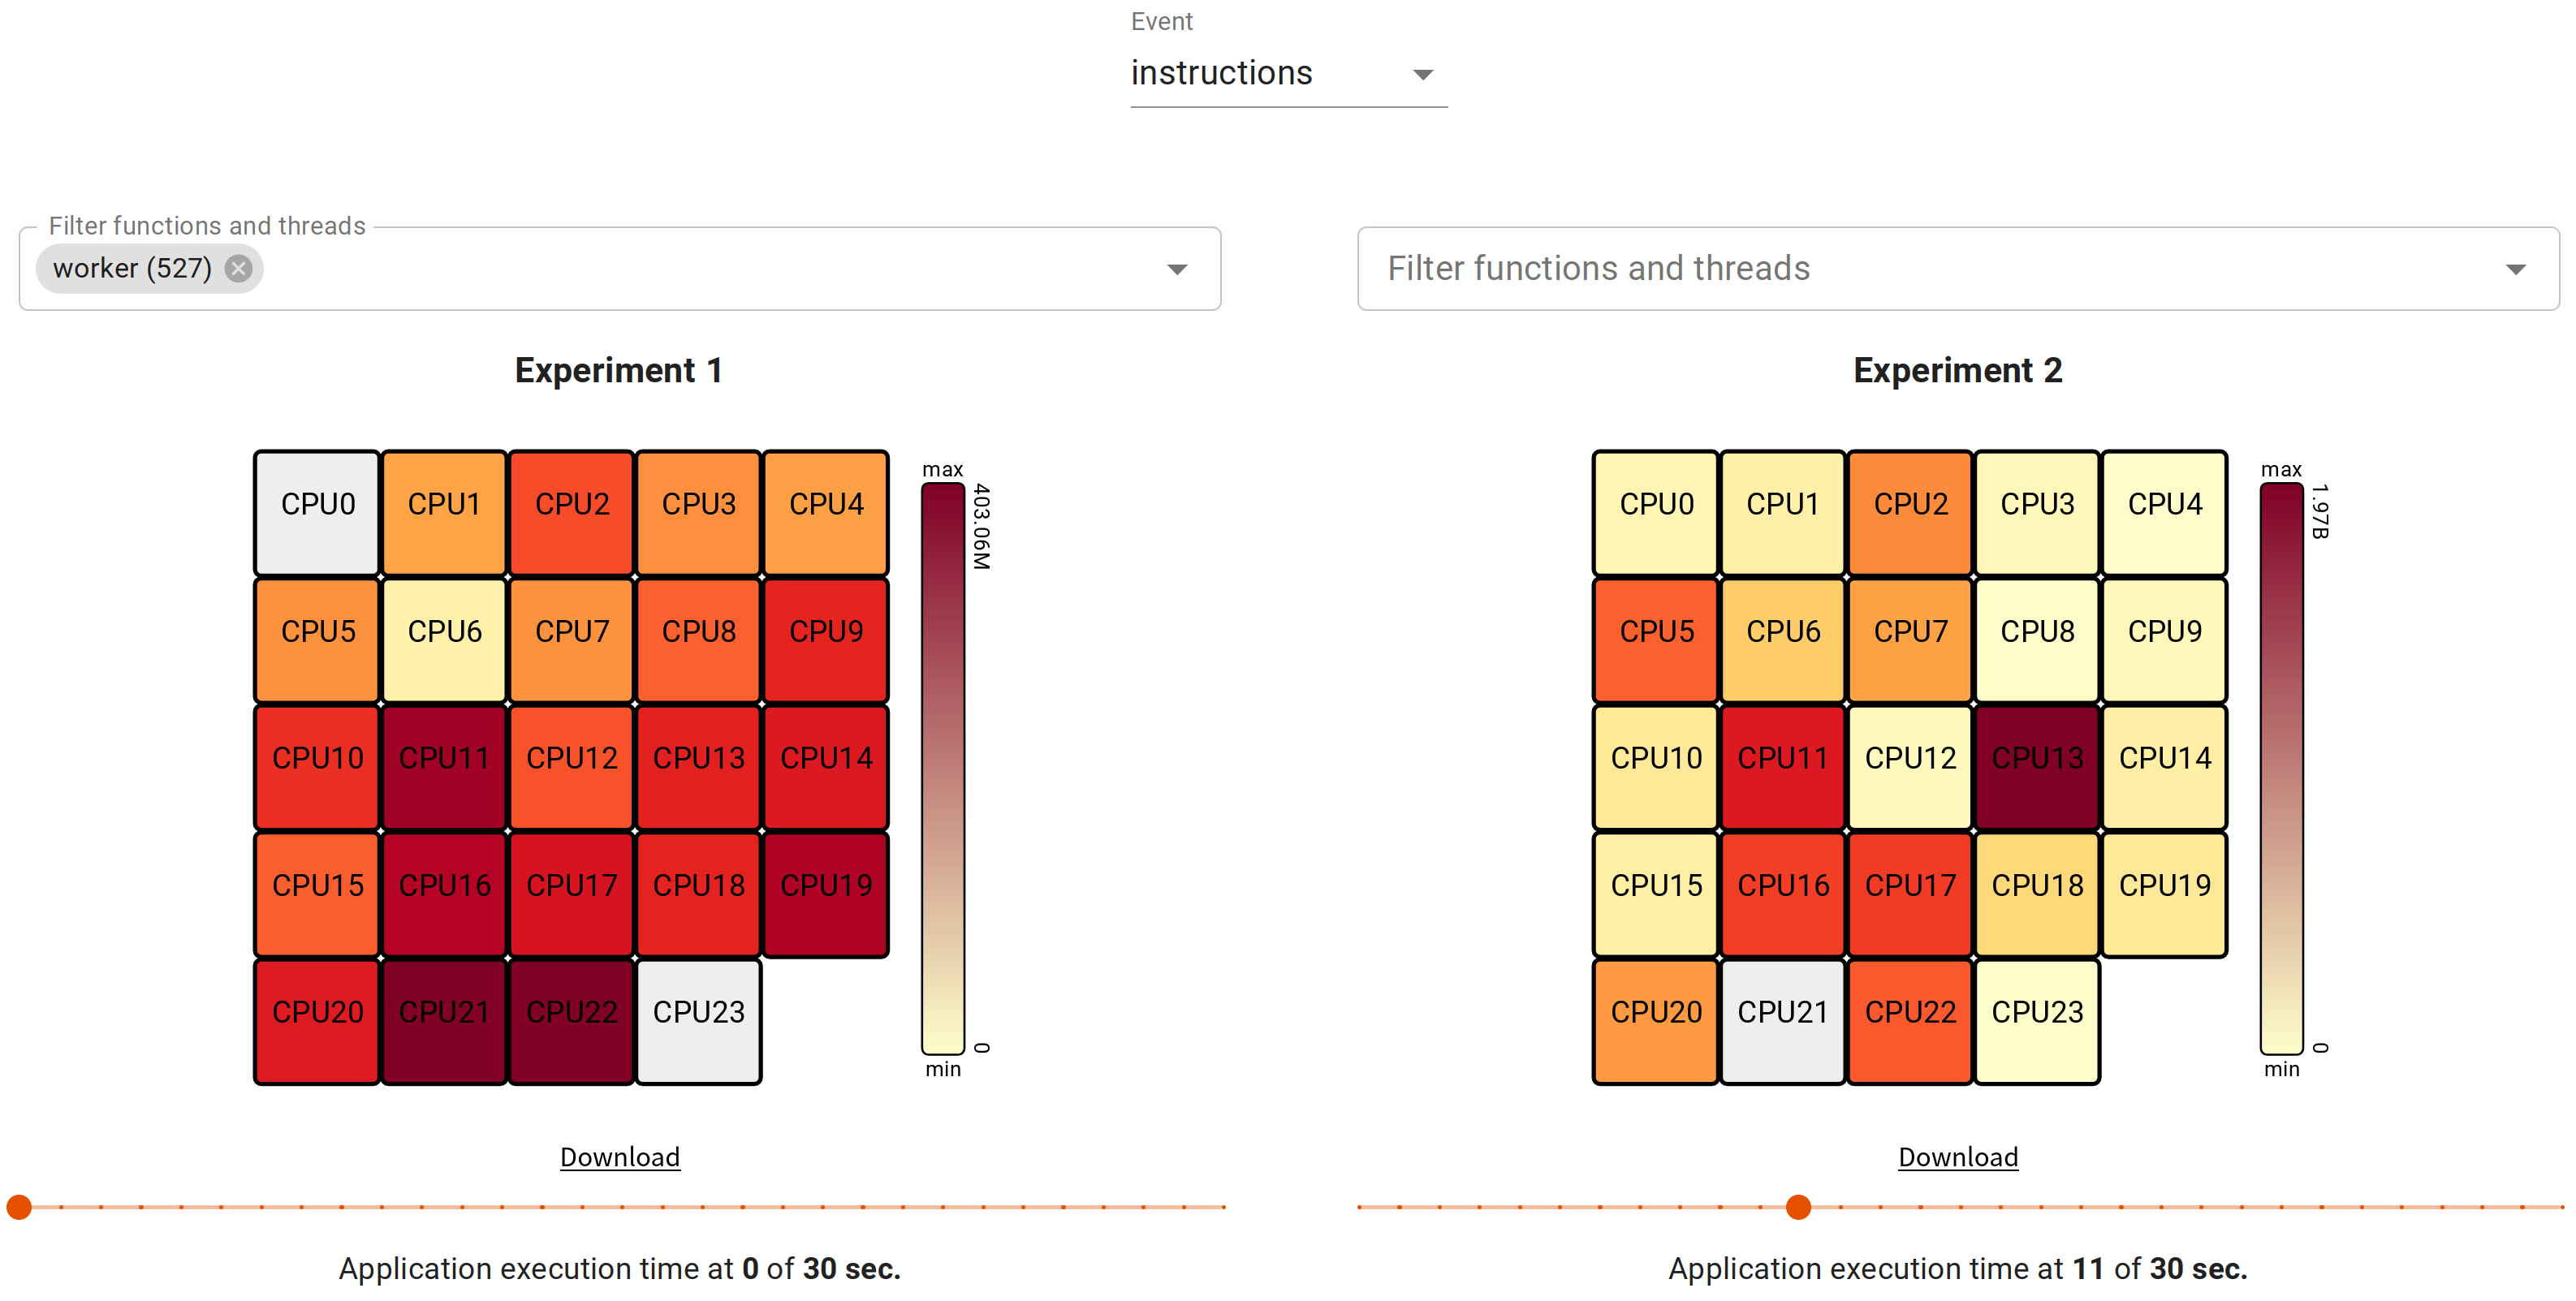
\includegraphics[width=1.0\columnwidth]{../pictures/visperf-section-2.png}
    \caption{VisPerf section ``Comparing experiments over execution time''.}
    \label{figure:visperf-section-2}
\end{figure}

The second section, named ``Comparing experiments over execution time'' and shown in Figure~\ref{figure:visperf-section-2}, allows to explore the performance of specific functions or threads executed in the program. Since Perf only output the thread id, we modified the application source code to output which was the function being executed in that specific threads. Therefore, thread ids that are not present in the program output are named as ``Other threads''. In this section, the user can see the performance of the PMUs at specific times of the application execution. Navigating in the experiment one, shown in Figure~\ref{figure:visperf-section-2}, we can see that CPUs 0 and 23 were not used. While in experiment two, all CPUs are used, and in some points some threads migrated of CPU while running the person recognition application. This behavior is correct because experiment one is using a fixed mapping, proposed by FastFlow, and experiment two the default mapping of the operating system.

Last section of VisPerf has metrics that use the events captured by Perf. For now, we only have one metrics: IPC (Instructions Per Cycle). This metric indicates the average number of instructions that were executed at each CPU cycle.

\begin{figure}
    \centering
    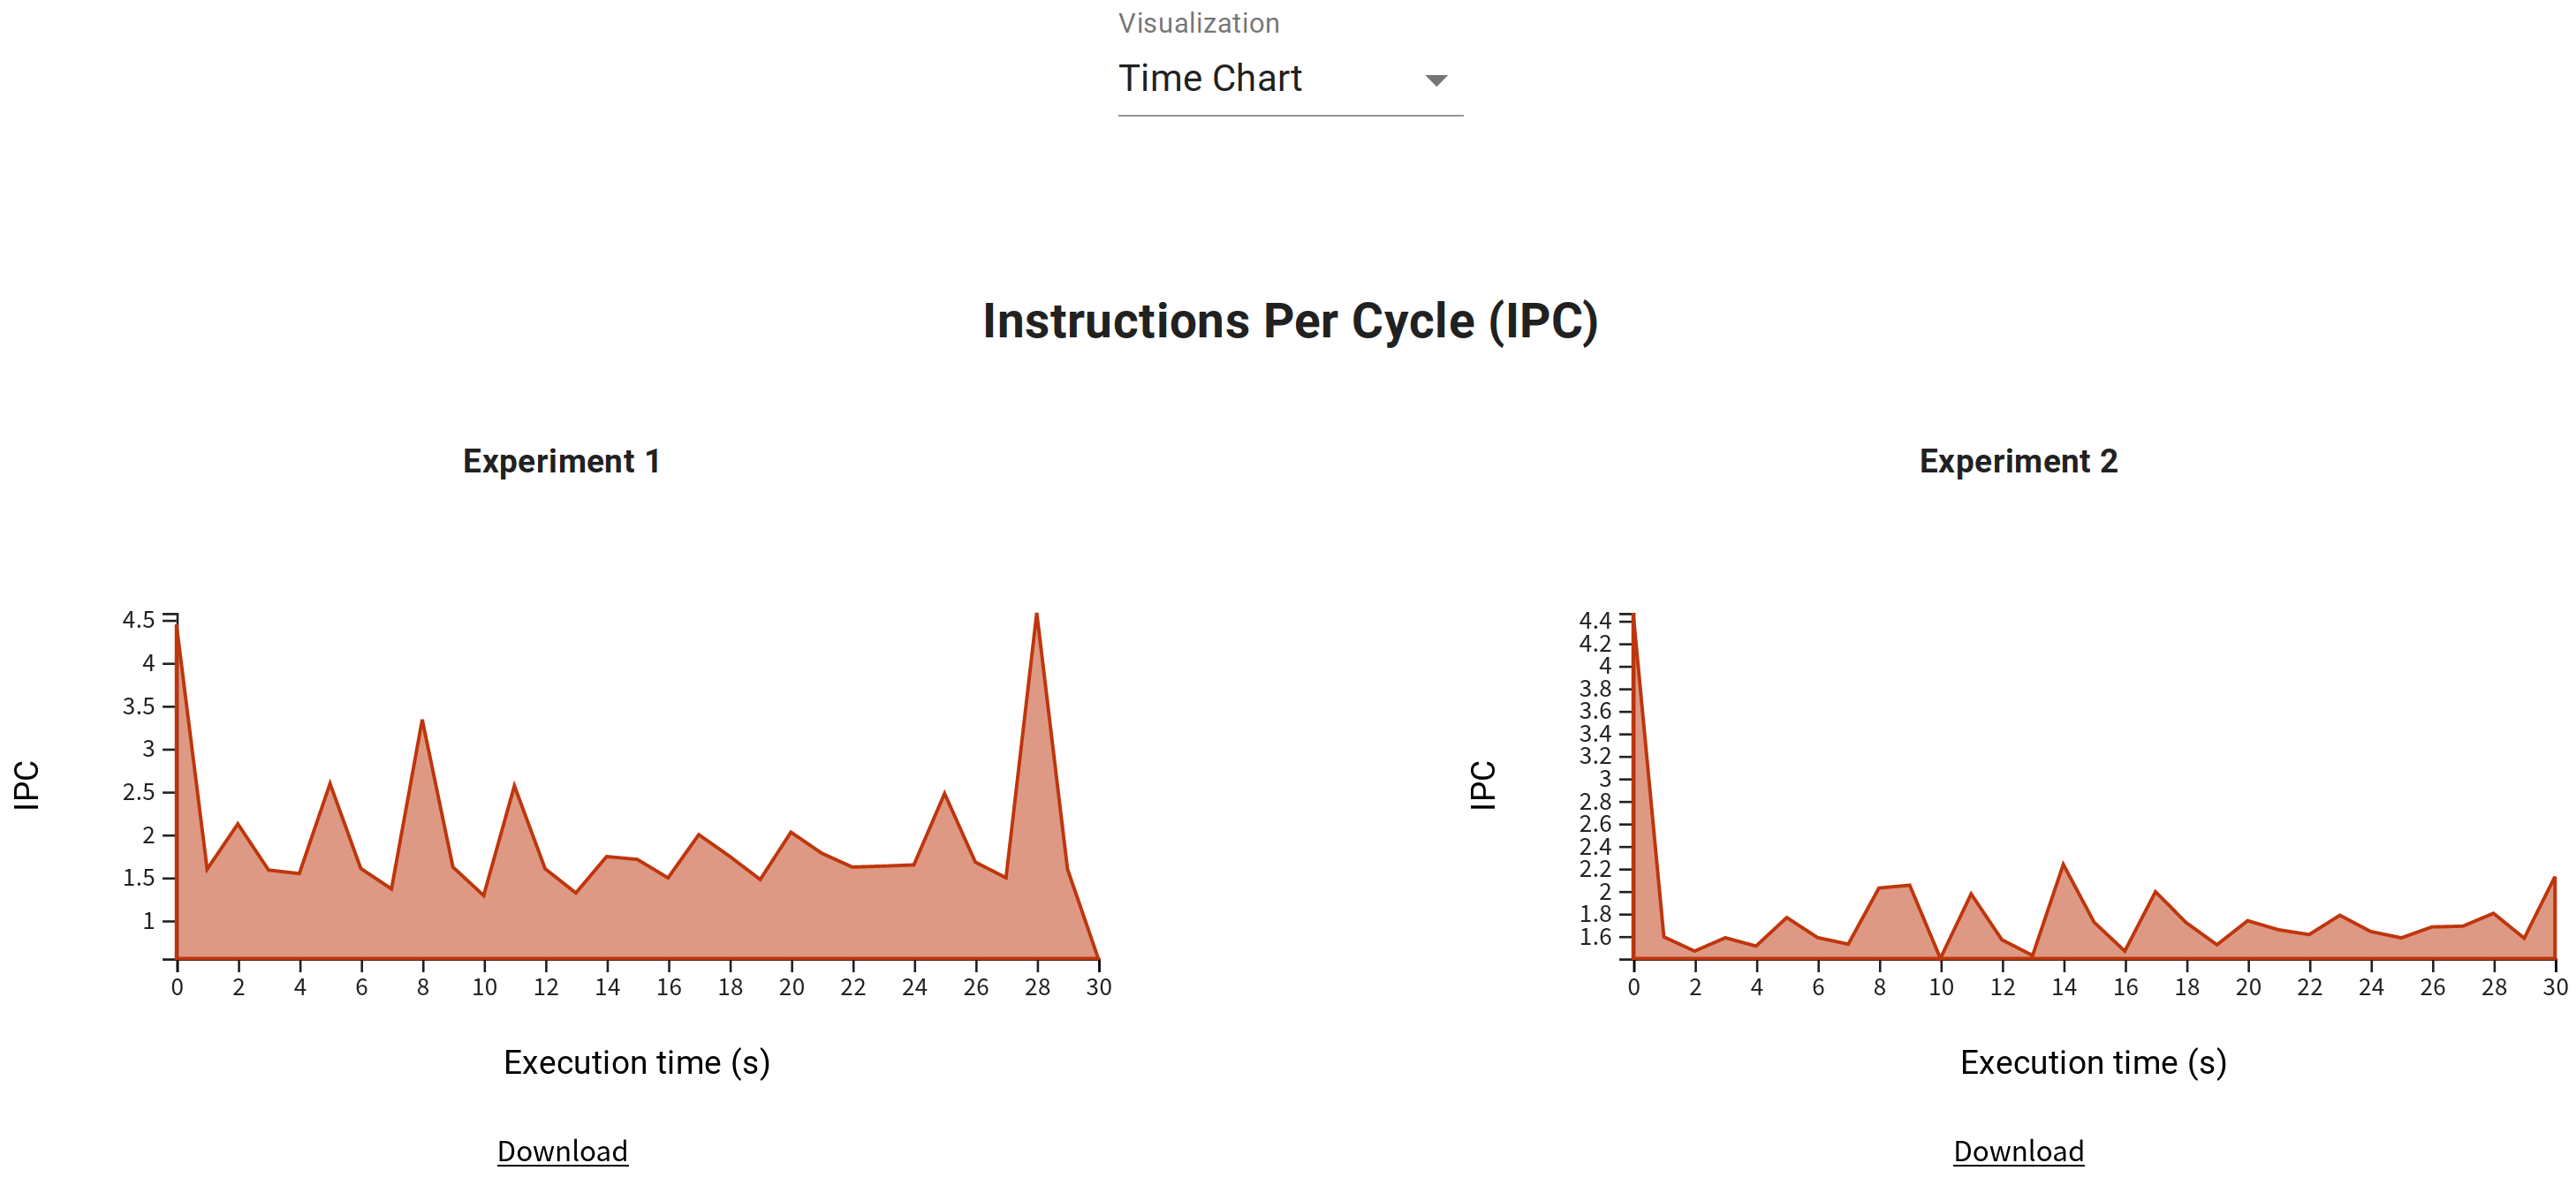
\includegraphics[width=1.0\columnwidth]{../pictures/visperf-section-3.png}
    \caption{VisPerf section ``Performance evaluation metrics''.}
    \label{figure:visperf-section-2}
\end{figure}
